% Options for packages loaded elsewhere
\PassOptionsToPackage{unicode}{hyperref}
\PassOptionsToPackage{hyphens}{url}
%
\documentclass[
  english,
  man]{apa7}
\title{The Effects of Zoom Self-View Distraction on Daily Self-Objectification and Well-Being}
\author{Randi L. Garcia\textsuperscript{1,2}, Jessica Pardim Araujo\textsuperscript{1}, Pamela Kramer\textsuperscript{1}, \& Sarah Bingham\textsuperscript{1}}
\date{}

\usepackage{amsmath,amssymb}
\usepackage{lmodern}
\usepackage{iftex}
\ifPDFTeX
  \usepackage[T1]{fontenc}
  \usepackage[utf8]{inputenc}
  \usepackage{textcomp} % provide euro and other symbols
\else % if luatex or xetex
  \usepackage{unicode-math}
  \defaultfontfeatures{Scale=MatchLowercase}
  \defaultfontfeatures[\rmfamily]{Ligatures=TeX,Scale=1}
\fi
% Use upquote if available, for straight quotes in verbatim environments
\IfFileExists{upquote.sty}{\usepackage{upquote}}{}
\IfFileExists{microtype.sty}{% use microtype if available
  \usepackage[]{microtype}
  \UseMicrotypeSet[protrusion]{basicmath} % disable protrusion for tt fonts
}{}
\makeatletter
\@ifundefined{KOMAClassName}{% if non-KOMA class
  \IfFileExists{parskip.sty}{%
    \usepackage{parskip}
  }{% else
    \setlength{\parindent}{0pt}
    \setlength{\parskip}{6pt plus 2pt minus 1pt}}
}{% if KOMA class
  \KOMAoptions{parskip=half}}
\makeatother
\usepackage{xcolor}
\IfFileExists{xurl.sty}{\usepackage{xurl}}{} % add URL line breaks if available
\IfFileExists{bookmark.sty}{\usepackage{bookmark}}{\usepackage{hyperref}}
\hypersetup{
  pdftitle={The Effects of Zoom Self-View Distraction on Daily Self-Objectification and Well-Being},
  pdfauthor={Randi L. Garcia1,2, Jessica Pardim Araujo1, Pamela Kramer1, \& Sarah Bingham1},
  pdflang={en-EN},
  pdfkeywords={keywords},
  hidelinks,
  pdfcreator={LaTeX via pandoc}}
\urlstyle{same} % disable monospaced font for URLs
\usepackage{graphicx}
\makeatletter
\def\maxwidth{\ifdim\Gin@nat@width>\linewidth\linewidth\else\Gin@nat@width\fi}
\def\maxheight{\ifdim\Gin@nat@height>\textheight\textheight\else\Gin@nat@height\fi}
\makeatother
% Scale images if necessary, so that they will not overflow the page
% margins by default, and it is still possible to overwrite the defaults
% using explicit options in \includegraphics[width, height, ...]{}
\setkeys{Gin}{width=\maxwidth,height=\maxheight,keepaspectratio}
% Set default figure placement to htbp
\makeatletter
\def\fps@figure{htbp}
\makeatother
\setlength{\emergencystretch}{3em} % prevent overfull lines
\providecommand{\tightlist}{%
  \setlength{\itemsep}{0pt}\setlength{\parskip}{0pt}}
\setcounter{secnumdepth}{-\maxdimen} % remove section numbering
% Make \paragraph and \subparagraph free-standing
\ifx\paragraph\undefined\else
  \let\oldparagraph\paragraph
  \renewcommand{\paragraph}[1]{\oldparagraph{#1}\mbox{}}
\fi
\ifx\subparagraph\undefined\else
  \let\oldsubparagraph\subparagraph
  \renewcommand{\subparagraph}[1]{\oldsubparagraph{#1}\mbox{}}
\fi
\newlength{\cslhangindent}
\setlength{\cslhangindent}{1.5em}
\newlength{\csllabelwidth}
\setlength{\csllabelwidth}{3em}
\newlength{\cslentryspacingunit} % times entry-spacing
\setlength{\cslentryspacingunit}{\parskip}
\newenvironment{CSLReferences}[2] % #1 hanging-ident, #2 entry spacing
 {% don't indent paragraphs
  \setlength{\parindent}{0pt}
  % turn on hanging indent if param 1 is 1
  \ifodd #1
  \let\oldpar\par
  \def\par{\hangindent=\cslhangindent\oldpar}
  \fi
  % set entry spacing
  \setlength{\parskip}{#2\cslentryspacingunit}
 }%
 {}
\usepackage{calc}
\newcommand{\CSLBlock}[1]{#1\hfill\break}
\newcommand{\CSLLeftMargin}[1]{\parbox[t]{\csllabelwidth}{#1}}
\newcommand{\CSLRightInline}[1]{\parbox[t]{\linewidth - \csllabelwidth}{#1}\break}
\newcommand{\CSLIndent}[1]{\hspace{\cslhangindent}#1}
% Manuscript styling
\usepackage{upgreek}
\captionsetup{font=singlespacing,justification=justified}

% Table formatting
\usepackage{longtable}
\usepackage{lscape}
% \usepackage[counterclockwise]{rotating}   % Landscape page setup for large tables
\usepackage{multirow}		% Table styling
\usepackage{tabularx}		% Control Column width
\usepackage[flushleft]{threeparttable}	% Allows for three part tables with a specified notes section
\usepackage{threeparttablex}            % Lets threeparttable work with longtable

% Create new environments so endfloat can handle them
% \newenvironment{ltable}
%   {\begin{landscape}\centering\begin{threeparttable}}
%   {\end{threeparttable}\end{landscape}}
\newenvironment{lltable}{\begin{landscape}\centering\begin{ThreePartTable}}{\end{ThreePartTable}\end{landscape}}

% Enables adjusting longtable caption width to table width
% Solution found at http://golatex.de/longtable-mit-caption-so-breit-wie-die-tabelle-t15767.html
\makeatletter
\newcommand\LastLTentrywidth{1em}
\newlength\longtablewidth
\setlength{\longtablewidth}{1in}
\newcommand{\getlongtablewidth}{\begingroup \ifcsname LT@\roman{LT@tables}\endcsname \global\longtablewidth=0pt \renewcommand{\LT@entry}[2]{\global\advance\longtablewidth by ##2\relax\gdef\LastLTentrywidth{##2}}\@nameuse{LT@\roman{LT@tables}} \fi \endgroup}

% \setlength{\parindent}{0.5in}
% \setlength{\parskip}{0pt plus 0pt minus 0pt}

% Overwrite redefinition of paragraph and subparagraph by the default LaTeX template
% See https://github.com/crsh/papaja/issues/292
\makeatletter
\renewcommand{\paragraph}{\@startsection{paragraph}{4}{\parindent}%
  {0\baselineskip \@plus 0.2ex \@minus 0.2ex}%
  {-1em}%
  {\normalfont\normalsize\bfseries\itshape\typesectitle}}

\renewcommand{\subparagraph}[1]{\@startsection{subparagraph}{5}{1em}%
  {0\baselineskip \@plus 0.2ex \@minus 0.2ex}%
  {-\z@\relax}%
  {\normalfont\normalsize\itshape\hspace{\parindent}{#1}\textit{\addperi}}{\relax}}
\makeatother

% \usepackage{etoolbox}
\makeatletter
\patchcmd{\HyOrg@maketitle}
  {\section{\normalfont\normalsize\abstractname}}
  {\section*{\normalfont\normalsize\abstractname}}
  {}{\typeout{Failed to patch abstract.}}
\patchcmd{\HyOrg@maketitle}
  {\section{\protect\normalfont{\@title}}}
  {\section*{\protect\normalfont{\@title}}}
  {}{\typeout{Failed to patch title.}}
\makeatother

\usepackage{xpatch}
\makeatletter
\xapptocmd\appendix
  {\xapptocmd\section
    {\addcontentsline{toc}{section}{\appendixname\ifoneappendix\else~\theappendix\fi\\: #1}}
    {}{\InnerPatchFailed}%
  }
{}{\PatchFailed}
\keywords{keywords\newline\indent Word count: Zoom, self-objectification, computer mediated communication, authenticity}
\DeclareDelayedFloatFlavor{ThreePartTable}{table}
\DeclareDelayedFloatFlavor{lltable}{table}
\DeclareDelayedFloatFlavor*{longtable}{table}
\makeatletter
\renewcommand{\efloat@iwrite}[1]{\immediate\expandafter\protected@write\csname efloat@post#1\endcsname{}}
\makeatother
\usepackage{csquotes}
\makeatletter
\renewcommand{\paragraph}{\@startsection{paragraph}{4}{\parindent}%
  {0\baselineskip \@plus 0.2ex \@minus 0.2ex}%
  {-1em}%
  {\normalfont\normalsize\bfseries\typesectitle}}

\renewcommand{\subparagraph}[1]{\@startsection{subparagraph}{5}{1em}%
  {0\baselineskip \@plus 0.2ex \@minus 0.2ex}%
  {-\z@\relax}%
  {\normalfont\normalsize\bfseries\itshape\hspace{\parindent}{#1}\textit{\addperi}}{\relax}}
\makeatother

\ifXeTeX
  % Load polyglossia as late as possible: uses bidi with RTL langages (e.g. Hebrew, Arabic)
  \usepackage{polyglossia}
  \setmainlanguage[]{english}
\else
  \usepackage[main=english]{babel}
% get rid of language-specific shorthands (see #6817):
\let\LanguageShortHands\languageshorthands
\def\languageshorthands#1{}
\fi
\ifLuaTeX
  \usepackage{selnolig}  % disable illegal ligatures
\fi


\shorttitle{Zoom and Self-Obejctification}

\authornote{

Smith College, Psychology Department, Smith College, Program in Statistical and Data Sciences.

The authors made the following contributions. Randi L. Garcia: Conceptualization, Methodology, Formal Analysis, Writing - Original Draft Preparation, Writing - Review \& Editing, Supervision; Jessica Pardim Araujo: Writing - Original Draft Preparation, Formal Analysis, Writing - Review \& Editing; Pamela Kramer: Formal Analysis, Writing - Review \& Editing; Sarah Bingham: Conceptualization, Methodology.

Correspondence concerning this article should be addressed to Randi L. Garcia, College Lane, Smith College, Northampton, MA 01063. E-mail: \href{mailto:rgarcia@smith.edu}{\nolinkurl{rgarcia@smith.edu}}

}

\affiliation{\vspace{0.5cm}\textsuperscript{1} Psychology Department, Smith College\\\textsuperscript{2} Program in Statistical and Data Sciences, Smith College}

\abstract{%
This study investigtaed the effects of using Zoom, specifically seeing oneself on Zoom on mental fatigue and general well-being.
}



\begin{document}
\maketitle

Zoom --\textgreater{} SSO --\textgreater{} Authenticity --\textgreater{} well-being (cognition, well-being)

\hypertarget{introduction-outline}{%
\section{Introduction Outline}\label{introduction-outline}}

\begin{enumerate}
\def\labelenumi{\arabic{enumi})}
\tightlist
\item
\end{enumerate}

\begin{itemize}
\tightlist
\item
  Problem
\item
  Literature

  \begin{itemize}
  \tightlist
  \item
    Zoom Fatigue
  \item
    Close paper on zoom and trait objectification
  \end{itemize}
\item
  Gap we are filling

  \begin{itemize}
  \tightlist
  \item
    5-day daily diaries
  \item
    State self-objectification
  \end{itemize}
\end{itemize}

\begin{enumerate}
\def\labelenumi{\arabic{enumi})}
\setcounter{enumi}{1}
\tightlist
\item
\end{enumerate}

\begin{itemize}
\tightlist
\item
  Computer mediated interaction and self-objectification

  \begin{itemize}
  \tightlist
  \item
    Social media
  \item
    Video chat (e.g Skype)
  \end{itemize}
\item
  State Self-Objectification

  \begin{itemize}
  \tightlist
  \item
    Authenticity
  \item
    Well-being and cognition
  \end{itemize}
\end{itemize}

\begin{enumerate}
\def\labelenumi{\arabic{enumi})}
\setcounter{enumi}{2}
\tightlist
\item
\end{enumerate}

\begin{itemize}
\tightlist
\item
  Zoom and well-being

  \begin{itemize}
  \tightlist
  \item
    Zoom fatigue
  \item
    Cognitive fatigue
  \end{itemize}
\end{itemize}

\begin{enumerate}
\def\labelenumi{\arabic{enumi})}
\setcounter{enumi}{3}
\tightlist
\item
\end{enumerate}

\begin{itemize}
\tightlist
\item
  Explaining reasons for the negative effects of Zoom

  \begin{itemize}
  \tightlist
  \item
    Self-objectification
  \item
    Seeing yourself
  \item
    Authenticity
  \item
    Studies on self-verification; studies using mirror.
  \end{itemize}
\end{itemize}

\begin{center}\rule{0.5\linewidth}{0.5pt}\end{center}

Teleworking and virtual meetings became the new reality for many individuals during the covid-19 lockdown. Although past research has shown video conferences as being positively correlated with higher productivity (Zornoza, Prieto, Martií \& Peiroó, 1993 ), switching from in-person interactions in the workplace or academic environment to spending a significant part of the day in virtual meetings has been linked to what it been called Virtual Meeting fatigue --- also known as Zoom fatigue (citation; Fosslien \& Duffy, 2020; Jiang, 2020). While Zoom fatigue can be defined as physical and mental exhaustion due to spending long hours exposed to this technology, Nadler (2020) points out that Zoom fatigue is more than just screen staring and argues that much of it is due to the visual complexities of interpersonal interactions. Additionally, Nadler (2020) also proposed the third skin concept, which explains how video conference members are ``flattened'' into a third skin composed of persons, background, and technology. Similarly, Bailenson (2021) discusses how the nonverbal overload that does not happen in an in-person meeting, such as excessive amounts of close-up eye gaze, cognitive load, increased self-evaluation from staring at a video of oneself, and constraints on physical mobility, could be a potential cause for fatigue and other psychological consequences such as negative self-evaluation and cognitive overload.

Studies have found women to be more susceptible to zoom fatigue than men. (Ratan, Miller \& Bailenson, J. N. 2022; Pfund GN, Hill PL, Harriger J, 2020; Shockley, K. M., Gabriel, A. S., Robertson, D., Rosen, C. C., Chawla, N., Ganster, M. L., \& Ezerins, M. E. 2021). Ratan et al.~(2022) study explain that facial dissatisfaction was found to be one of the reasons for higher zoom fatigue in women. Additionally, due to the possibility of being able to see oneself on screen, self-objectification was found to be another possible explanation of higher zoom fatigue, especially in women (Luo, Queiroz, Bailenson, Hancock, 2021; Pfund GN, Hill PL, Harriger J, 2020). In this study, we look into daily zoom use and how being distracted by one's self-image through the self-view feature can increase the state of self-objectification in young women. Through a five-day daily diary, we investigate how zoom was related to authenticity and daily well-being. Moreover, this is the first study to explore trait self-objectification as a moderator of zoom usage and state self-objectification.

\hypertarget{social-media-and-self-objectification}{%
\section{Social Media and Self-Objectification}\label{social-media-and-self-objectification}}

While there is a lack of self-objectification and other video chat interactions, such as skype, self-objectification in magazines, television and social media is a vast researched topic that can help us understand computer-mediated interactions relationship with self-objectification. Frederick and Robberts (1997) presented the objectification theory and defined self-objectification as feeling more like a body or an object rather than a human being. Past research has found that time spent on social media usage (e.g., Instagram, Facebook, Snapchat) and the use of its features (e.g., filter, likes, comments) are positively correlated to body dissatisfaction, eating disorders, appearance comparison, and self-objectification ( Bell, B. T., Cassarly, J. A., \& Dunbar, L. 2018; Fardouly et al., 2015; Garcia, Bingham, \& Liu 2021; Hanna et al., 2017; Pfund, Hill, and Harriger, 2020). Even though time was a predictor of self-objectification on social media, the same did not apply to Zoom. For instance, Harriger \& Pfund (2022) found that the more time men and women spent on Zoom, the more appearance satisfaction was reported. However, the amount of time one spent looking at oneself was associated with appearance comparison and self-objectification. Thus, we could argue that being able to see oneself during video conferences could lead to social comparison with one's image throughout the day and negative self-attention, which could increase Zoom fatigue.

State self-objectification (SSO) is a context-dependent condition that is triggered depending on the situation, for example, seeing sexualized images on social media or getting catcalled on the street. Trait self-objectification (TSO) is the internalized self-objectification throughout the years. Additionally, someone high in TSO is more prone to SSO (Fredrickson \& Roberts, 1997; Gay \& Castano, 2010). There are numerous cognitive and psychological consequences of being objectified. Even though some studies have shown that men are also self-objectifiers (see Daniel, Bridges, \& Martens, 2014), women have more damaging and long-lasting consequences (Jones \& Griffiths, 2015). For instance, studies have found that participants who present higher objectification reported feeling less authentic and having lower levels of subjective well-being in both workplace and academic settings (Cheng et al., 2022; Rollero, 2016).
\emph{add swimsuit study}

Additionally, Pfund, Hill, Harriger (2020) while using self-objectification as a moderator, found that being able to see oneself during a video call can increase ones self-objectification.

\emph{use of the self-view feature has been linked to Being able to see oneself during meetings is also a door that leads to negative self-attention known as mirror anxiety.}

\hypertarget{zoom-and-well-being}{%
\section{Zoom and well-being}\label{zoom-and-well-being}}

In the past years, researchers have been investigating the reasons that lead to zoom fatigue. For instance, Zoom meetings, differently from in-person, feature the possibility of looking at oneself during video calls through the feature known as ``self-view.'' Hence, because people are not used to viewing themselves when talking to others, the self-view feature can trigger thoughts and feelings that were not previously possible during in-person interactions and thus increasing fatigue (Fauville, G., Luo, M., Queiroz, A. C. M., Bailenson, J. N., \& Hancock, J. 2021; Shockley, K. M., Gabriel, A. S., Robertson, D., Rosen, C. C., Chawla, N., Ganster, M. L., \& Ezerins, M. E. 2021; Bailenson, J. N. 2021) ).

Ratan, Miller, and Bailenson (2022) explain how negative self-focused attention, known as mirror anxiety, leads to facial dissatisfaction and consequently increases Zoom fatigue.

\hypertarget{zoom-negative-effects}{%
\section{Zoom negative effects}\label{zoom-negative-effects}}

For instance, Ratan, Miller, and Bailenson (2022), explains how negative self-focused attention, known as mirror anxiety, leads to facial dissatisfaction and consequently increases Zoom fatigue.

Past studies have found that using Zoom can cause mental fatigue (Bailenson, 2021). Seeing oneself on Zoom has also been linked to appearance concerns (Pfund et al., 2020).

\hypertarget{methods}{%
\section{Methods}\label{methods}}

\hypertarget{participants}{%
\subsection{Participants}\label{participants}}

\hypertarget{measures}{%
\subsection{Measures}\label{measures}}

\hypertarget{procedure}{%
\subsection{Procedure}\label{procedure}}

\hypertarget{data-analysis}{%
\subsection{Data analysis}\label{data-analysis}}

We used R (Version 4.1.2; R Core Team, 2022) and the R-packages \emph{dplyr} (Version 1.0.9; Wickham et al., 2021), \emph{forcats} (Version 0.5.1; Wickham, 2021a), \emph{ggplot2} (Version 3.3.6; Wickham, 2016), \emph{lme4} (Version 1.1.27.1; Bates et al., 2015), \emph{lmerTest} (Version 3.1.3; Kuznetsova et al., 2017), \emph{Matrix} (Version 1.3.4; Bates \& Maechler, 2021), \emph{nlme} (Version 3.1.153; Pinheiro et al., 2021), \emph{papaja} (Version 0.1.0.9999; Aust \& Barth, 2022), \emph{psych} (Version 2.1.9; Revelle, 2021), \emph{purrr} (Version 0.3.4; Henry \& Wickham, 2020), \emph{readr} (Version 2.1.0; Wickham \& Hester, 2020), \emph{stringr} (Version 1.4.0; Wickham, 2019), \emph{tibble} (Version 3.1.7; Müller \& Wickham, 2021), \emph{tidyr} (Version 1.2.0; Wickham, 2021b), \emph{tidyverse} (Version 1.3.1; Wickham et al., 2019), and \emph{tinylabels} (Version 0.2.3; Barth, 2022) for all our analyses.

\hypertarget{results}{%
\section{Results}\label{results}}

\hypertarget{zoom-use-and-state-self-objectification}{%
\subsection{Zoom Use and State Self-Objectification}\label{zoom-use-and-state-self-objectification}}

\begin{verbatim}
##                          daily_SSO daily_SSO_binary    tso_mean     OBCS_sur
## daily_SSO               1.00000000      0.669651633  0.03813339  0.129034893
## daily_SSO_binary        0.66965163      1.000000000  0.08455927  0.133948249
## tso_mean                0.03813339      0.084559269  1.00000000  0.509816730
## OBCS_sur                0.12903489      0.133948249  0.50981673  1.000000000
## SPA                     0.01420422     -0.004678395  0.38593126  0.635991331
## Zoom_Total_Mins         0.11366899      0.098484033 -0.09266711 -0.132232776
## Zoom_Use_Weekly         0.07773376     -0.031371983 -0.18508483 -0.126526116
## Zoom_Use_Daily          0.10571735     -0.027760827  0.06465371 -0.127190827
## Hide_Self_View         -0.02587184      0.198546362  0.12282535 -0.004671422
## Image_Distraction       0.10010665     -0.007788432  0.14806292  0.117445719
## Hide_Self_View_Today    0.21461607      0.378339881  0.15627801  0.005227725
## Self_Distraction_Today  0.32458884      0.196644793  0.14656102  0.132867310
##                                 SPA Zoom_Total_Mins Zoom_Use_Weekly
## daily_SSO               0.014204220     0.113668986      0.07773376
## daily_SSO_binary       -0.004678395     0.098484033     -0.03137198
## tso_mean                0.385931258    -0.092667107     -0.18508483
## OBCS_sur                0.635991331    -0.132232776     -0.12652612
## SPA                     1.000000000    -0.006451003     -0.22790376
## Zoom_Total_Mins        -0.006451003     1.000000000      0.06138500
## Zoom_Use_Weekly        -0.227903761     0.061385004      1.00000000
## Zoom_Use_Daily          0.042908228     0.130753584      0.13082707
## Hide_Self_View          0.173510410    -0.089828387     -0.27143195
## Image_Distraction       0.156316498     0.026528390     -0.01306277
## Hide_Self_View_Today    0.041093694    -0.049584763     -0.20875119
## Self_Distraction_Today  0.194822268     0.315559981      0.03132817
##                        Zoom_Use_Daily Hide_Self_View Image_Distraction
## daily_SSO                  0.10571735   -0.025871843       0.100106650
## daily_SSO_binary          -0.02776083    0.198546362      -0.007788432
## tso_mean                   0.06465371    0.122825347       0.148062916
## OBCS_sur                  -0.12719083   -0.004671422       0.117445719
## SPA                        0.04290823    0.173510410       0.156316498
## Zoom_Total_Mins            0.13075358   -0.089828387       0.026528390
## Zoom_Use_Weekly            0.13082707   -0.271431951      -0.013062770
## Zoom_Use_Daily             1.00000000    0.077320990      -0.088831855
## Hide_Self_View             0.07732099    1.000000000      -0.099508355
## Image_Distraction         -0.08883186   -0.099508355       1.000000000
## Hide_Self_View_Today      -0.01076344    0.529907315      -0.125012753
## Self_Distraction_Today    -0.02025397   -0.110297677       0.509468540
##                        Hide_Self_View_Today Self_Distraction_Today
## daily_SSO                       0.214616070             0.32458884
## daily_SSO_binary                0.378339881             0.19664479
## tso_mean                        0.156278013             0.14656102
## OBCS_sur                        0.005227725             0.13286731
## SPA                             0.041093694             0.19482227
## Zoom_Total_Mins                -0.049584763             0.31555998
## Zoom_Use_Weekly                -0.208751187             0.03132817
## Zoom_Use_Daily                 -0.010763438            -0.02025397
## Hide_Self_View                  0.529907315            -0.11029768
## Image_Distraction              -0.125012753             0.50946854
## Hide_Self_View_Today            1.000000000            -0.07263685
## Self_Distraction_Today         -0.072636848             1.00000000
\end{verbatim}

\begin{verbatim}
## Generalized linear mixed model fit by maximum likelihood (Laplace
##   Approximation) [glmerMod]
##  Family: binomial  ( logit )
## Formula: daily_SSO_binary ~ day + Zoom_Total_Mins + (1 | partID)
##    Data: zoom_clean
## 
##      AIC      BIC   logLik deviance df.resid 
##    185.2    197.6    -88.6    177.2      162 
## 
## Scaled residuals: 
##     Min      1Q  Median      3Q     Max 
## -3.2469 -0.4428  0.2167  0.3968  2.0676 
## 
## Random effects:
##  Groups Name        Variance Std.Dev.
##  partID (Intercept) 6.005    2.451   
## Number of obs: 166, groups:  partID, 37
## 
## Fixed effects:
##                  Estimate Std. Error z value Pr(>|z|)  
## (Intercept)      1.388783   0.878402   1.581   0.1139  
## day             -0.298014   0.177565  -1.678   0.0933 .
## Zoom_Total_Mins  0.002662   0.002428   1.096   0.2730  
## ---
## Signif. codes:  0 '***' 0.001 '**' 0.01 '*' 0.05 '.' 0.1 ' ' 1
## 
## Correlation of Fixed Effects:
##             (Intr) day   
## day         -0.743       
## Zom_Ttl_Mns -0.519  0.248
\end{verbatim}

\begin{verbatim}
## Linear mixed model fit by REML. t-tests use Satterthwaite's method [
## lmerModLmerTest]
## Formula: daily_SSO ~ day + Zoom_Total_Mins + (1 | partID)
##    Data: zoom_clean
## 
## REML criterion at convergence: 597.9
## 
## Scaled residuals: 
##     Min      1Q  Median      3Q     Max 
## -1.8641 -0.4788 -0.1423  0.3692  3.7354 
## 
## Random effects:
##  Groups   Name        Variance Std.Dev.
##  partID   (Intercept) 1.533    1.238   
##  Residual             1.324    1.150   
## Number of obs: 166, groups:  partID, 37
## 
## Fixed effects:
##                   Estimate Std. Error         df t value Pr(>|t|)    
## (Intercept)      2.536e+00  3.570e-01  1.293e+02   7.103 7.29e-11 ***
## day             -1.085e-01  6.839e-02  1.331e+02  -1.586    0.115    
## Zoom_Total_Mins  1.137e-03  9.174e-04  1.510e+02   1.239    0.217    
## ---
## Signif. codes:  0 '***' 0.001 '**' 0.01 '*' 0.05 '.' 0.1 ' ' 1
## 
## Correlation of Fixed Effects:
##             (Intr) day   
## day         -0.691       
## Zom_Ttl_Mns -0.565  0.329
\end{verbatim}

\begin{verbatim}
## Linear mixed model fit by REML. t-tests use Satterthwaite's method [
## lmerModLmerTest]
## Formula: daily_SSO ~ day + Hide_Self_View_Today + Self_Distraction_Today +  
##     (1 | partID)
##    Data: zoom_clean
## 
## REML criterion at convergence: 594.2
## 
## Scaled residuals: 
##     Min      1Q  Median      3Q     Max 
## -2.1665 -0.4526 -0.1679  0.3987  3.9458 
## 
## Random effects:
##  Groups   Name        Variance Std.Dev.
##  partID   (Intercept) 1.279    1.131   
##  Residual             1.251    1.118   
## Number of obs: 171, groups:  partID, 37
## 
## Fixed effects:
##                         Estimate Std. Error        df t value Pr(>|t|)    
## (Intercept)              1.57159    0.45032 150.76703   3.490 0.000634 ***
## day                     -0.08087    0.06425 136.43794  -1.259 0.210315    
## Hide_Self_View_Today     0.25845    0.08948 166.58432   2.888 0.004386 ** 
## Self_Distraction_Today   0.20793    0.09968 166.50076   2.086 0.038502 *  
## ---
## Signif. codes:  0 '***' 0.001 '**' 0.01 '*' 0.05 '.' 0.1 ' ' 1
## 
## Correlation of Fixed Effects:
##             (Intr) day    H_S_V_
## day         -0.598              
## Hd_Slf_Vw_T -0.478  0.070       
## Slf_Dstrc_T -0.658  0.289  0.053
\end{verbatim}

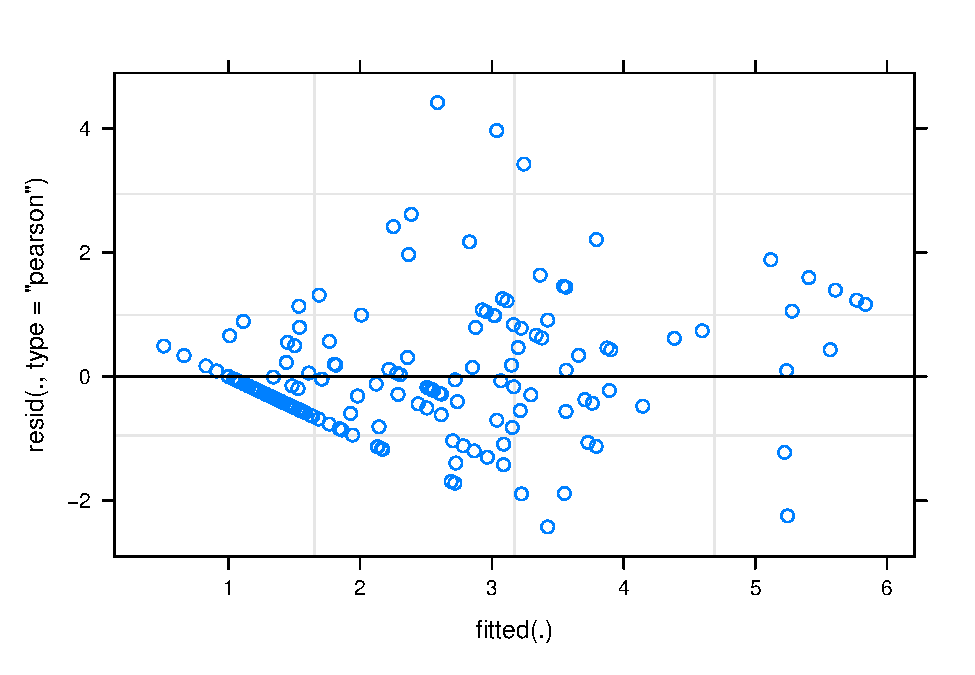
\includegraphics{zoom_sso_manuscript_files/figure-latex/unnamed-chunk-3-1.pdf}

\begin{verbatim}
## Generalized linear mixed model fit by maximum likelihood (Laplace
##   Approximation) [glmerMod]
##  Family: binomial  ( logit )
## Formula: 
## daily_SSO_binary ~ day + Hide_Self_View_Today + Self_Distraction_Today +  
##     (1 | partID)
##    Data: zoom_clean
## 
##      AIC      BIC   logLik deviance df.resid 
##    175.8    191.6    -82.9    165.8      166 
## 
## Scaled residuals: 
##     Min      1Q  Median      3Q     Max 
## -3.9434 -0.4074  0.1714  0.3408  2.5391 
## 
## Random effects:
##  Groups Name        Variance Std.Dev.
##  partID (Intercept) 4.499    2.121   
## Number of obs: 171, groups:  partID, 37
## 
## Fixed effects:
##                        Estimate Std. Error z value Pr(>|z|)   
## (Intercept)             -1.5033     1.1116  -1.352  0.17626   
## day                     -0.2198     0.1733  -1.268  0.20471   
## Hide_Self_View_Today     0.8500     0.2601   3.268  0.00108 **
## Self_Distraction_Today   0.5396     0.2697   2.001  0.04536 * 
## ---
## Signif. codes:  0 '***' 0.001 '**' 0.01 '*' 0.05 '.' 0.1 ' ' 1
## 
## Correlation of Fixed Effects:
##             (Intr) day    H_S_V_
## day         -0.584              
## Hd_Slf_Vw_T -0.478 -0.008       
## Slf_Dstrc_T -0.654  0.169  0.110
\end{verbatim}

Interaction with TSO

\begin{verbatim}
## Generalized linear mixed model fit by maximum likelihood (Laplace
##   Approximation) [glmerMod]
##  Family: binomial  ( logit )
## Formula: 
## daily_SSO_binary ~ day + Hide_Self_View_Today * OBCS_sur + Self_Distraction_Today *  
##     OBCS_sur + (1 | partID)
##    Data: zoom_clean
## 
##      AIC      BIC   logLik deviance df.resid 
##    179.9    205.1    -82.0    163.9      163 
## 
## Scaled residuals: 
##     Min      1Q  Median      3Q     Max 
## -3.3900 -0.4136  0.1623  0.3529  2.8225 
## 
## Random effects:
##  Groups Name        Variance Std.Dev.
##  partID (Intercept) 4.147    2.036   
## Number of obs: 171, groups:  partID, 37
## 
## Fixed effects:
##                                 Estimate Std. Error z value Pr(>|z|)
## (Intercept)                     -0.23466    4.00808  -0.059    0.953
## day                             -0.21474    0.17395  -1.234    0.217
## Hide_Self_View_Today             0.51887    1.10773   0.468    0.639
## OBCS_sur                        -0.25230    0.79716  -0.317    0.752
## Self_Distraction_Today          -0.56981    1.20541  -0.473    0.636
## Hide_Self_View_Today:OBCS_sur    0.07135    0.22232   0.321    0.748
## OBCS_sur:Self_Distraction_Today  0.21906    0.23631   0.927    0.354
## 
## Correlation of Fixed Effects:
##             (Intr) day    Hd_S_V_T OBCS_s Sl_D_T H_S_V_T:
## day         -0.153                                       
## Hd_Slf_Vw_T -0.554 -0.050                                
## OBCS_sur    -0.961 -0.012  0.555                         
## Slf_Dstrc_T -0.687  0.086  0.020    0.661                
## H_S_V_T:OBC  0.540  0.050 -0.971   -0.573 -0.032         
## OBCS_:S_D_T  0.680 -0.046 -0.041   -0.696 -0.975  0.059
\end{verbatim}

\begin{verbatim}
## Generalized linear mixed model fit by maximum likelihood (Laplace
##   Approximation) [glmerMod]
##  Family: binomial  ( logit )
## Formula: 
## daily_SSO_binary ~ day + Hide_Self_View_Today + Self_Distraction_Today +  
##     OBCS_sur + (1 | partID)
##    Data: zoom_clean
## 
##      AIC      BIC   logLik deviance df.resid 
##    176.8    195.7    -82.4    164.8      165 
## 
## Scaled residuals: 
##     Min      1Q  Median      3Q     Max 
## -3.8015 -0.4224  0.1822  0.3380  2.5084 
## 
## Random effects:
##  Groups Name        Variance Std.Dev.
##  partID (Intercept) 4.286    2.07    
## Number of obs: 171, groups:  partID, 37
## 
## Fixed effects:
##                        Estimate Std. Error z value Pr(>|z|)    
## (Intercept)             -3.3770     2.1752  -1.553  0.12054    
## day                     -0.2156     0.1731  -1.246  0.21285    
## Hide_Self_View_Today     0.8580     0.2605   3.293  0.00099 ***
## Self_Distraction_Today   0.5263     0.2685   1.960  0.04996 *  
## OBCS_sur                 0.3869     0.3887   0.995  0.31957    
## ---
## Signif. codes:  0 '***' 0.001 '**' 0.01 '*' 0.05 '.' 0.1 ' ' 1
## 
## Correlation of Fixed Effects:
##             (Intr) day    H_S_V_ Sl_D_T
## day         -0.276                     
## Hd_Slf_Vw_T -0.311 -0.003              
## Slf_Dstrc_T -0.311  0.168  0.106       
## OBCS_sur    -0.861 -0.026  0.077 -0.023
\end{verbatim}

\begin{verbatim}
## Generalized linear mixed model fit by maximum likelihood (Laplace
##   Approximation) [glmerMod]
##  Family: binomial  ( logit )
## Formula: 
## daily_SSO_binary ~ day + Hide_Self_View_Today * tso_mean + Self_Distraction_Today *  
##     tso_mean + (1 | partID)
##    Data: zoom_clean
## 
##      AIC      BIC   logLik deviance df.resid 
##    179.0    204.1    -81.5    163.0      163 
## 
## Scaled residuals: 
##     Min      1Q  Median      3Q     Max 
## -2.8700 -0.3829  0.1576  0.3273  2.1989 
## 
## Random effects:
##  Groups Name        Variance Std.Dev.
##  partID (Intercept) 4.967    2.229   
## Number of obs: 171, groups:  partID, 37
## 
## Fixed effects:
##                                 Estimate Std. Error z value Pr(>|z|)   
## (Intercept)                     -1.51922    1.16519  -1.304  0.19229   
## day                             -0.22457    0.17839  -1.259  0.20808   
## Hide_Self_View_Today             0.84200    0.27195   3.096  0.00196 **
## tso_mean                        -0.46605    0.35265  -1.322  0.18631   
## Self_Distraction_Today           0.52544    0.27997   1.877  0.06055 . 
## Hide_Self_View_Today:tso_mean    0.07775    0.10703   0.726  0.46753   
## tso_mean:Self_Distraction_Today  0.15808    0.10825   1.460  0.14417   
## ---
## Signif. codes:  0 '***' 0.001 '**' 0.01 '*' 0.05 '.' 0.1 ' ' 1
## 
## Correlation of Fixed Effects:
##             (Intr) day    Hd_S_V_T tso_mn Sl_D_T H_S_V_T:
## day         -0.561                                       
## Hd_Slf_Vw_T -0.490 -0.018                                
## tso_mean     0.094  0.079 -0.086                         
## Slf_Dstrc_T -0.663  0.163  0.123   -0.108                
## Hd_Sl_V_T:_ -0.021 -0.032 -0.032   -0.589  0.076         
## ts_mn:S_D_T -0.037 -0.087  0.085   -0.698  0.034  0.076
\end{verbatim}

\begin{verbatim}
## Generalized linear mixed model fit by maximum likelihood (Laplace
##   Approximation) [glmerMod]
##  Family: binomial  ( logit )
## Formula: 
## daily_SSO_binary ~ day + Hide_Self_View_Today + Self_Distraction_Today +  
##     tso_mean + (1 | partID)
##    Data: zoom_clean
## 
##      AIC      BIC   logLik deviance df.resid 
##    177.8    196.7    -82.9    165.8      165 
## 
## Scaled residuals: 
##     Min      1Q  Median      3Q     Max 
## -3.9275 -0.4084  0.1716  0.3402  2.5375 
## 
## Random effects:
##  Groups Name        Variance Std.Dev.
##  partID (Intercept) 4.501    2.122   
## Number of obs: 171, groups:  partID, 37
## 
## Fixed effects:
##                         Estimate Std. Error z value Pr(>|z|)   
## (Intercept)            -1.496381   1.120484  -1.335  0.18172   
## day                    -0.219685   0.173288  -1.268  0.20489   
## Hide_Self_View_Today    0.848529   0.261710   3.242  0.00119 **
## Self_Distraction_Today  0.538329   0.270928   1.987  0.04692 * 
## tso_mean                0.007804   0.159002   0.049  0.96085   
## ---
## Signif. codes:  0 '***' 0.001 '**' 0.01 '*' 0.05 '.' 0.1 ' ' 1
## 
## Correlation of Fixed Effects:
##             (Intr) day    H_S_V_ Sl_D_T
## day         -0.579                     
## Hd_Slf_Vw_T -0.485 -0.008              
## Slf_Dstrc_T -0.658  0.168  0.120       
## tso_mean     0.126  0.006 -0.110 -0.097
\end{verbatim}

\begin{verbatim}
## Generalized linear mixed model fit by maximum likelihood (Laplace
##   Approximation) [glmerMod]
##  Family: binomial  ( logit )
## Formula: 
## daily_SSO_binary ~ day + Hide_Self_View_Today + Self_Distraction_Today *  
##     SPA + (1 | partID)
##    Data: zoom_clean
## 
##      AIC      BIC   logLik deviance df.resid 
##    177.9    199.9    -82.0    163.9      164 
## 
## Scaled residuals: 
##     Min      1Q  Median      3Q     Max 
## -2.8579 -0.4136  0.1594  0.3368  2.8075 
## 
## Random effects:
##  Groups Name        Variance Std.Dev.
##  partID (Intercept) 4.253    2.062   
## Number of obs: 171, groups:  partID, 37
## 
## Fixed effects:
##                            Estimate Std. Error z value Pr(>|z|)    
## (Intercept)                  2.2378     3.1856   0.702 0.482381    
## day                         -0.2225     0.1740  -1.278 0.201102    
## Hide_Self_View_Today         0.8753     0.2646   3.308 0.000939 ***
## Self_Distraction_Today      -1.0016     1.1613  -0.863 0.388403    
## SPA                         -1.1204     0.8969  -1.249 0.211579    
## Self_Distraction_Today:SPA   0.4490     0.3328   1.349 0.177281    
## ---
## Signif. codes:  0 '***' 0.001 '**' 0.01 '*' 0.05 '.' 0.1 ' ' 1
## 
## Correlation of Fixed Effects:
##             (Intr) day    H_S_V_ Sl_D_T SPA   
## day         -0.256                            
## Hd_Slf_Vw_T -0.066 -0.028                     
## Slf_Dstrc_T -0.777  0.110 -0.098              
## SPA         -0.937  0.059 -0.106  0.774       
## Slf_D_T:SPA  0.754 -0.074  0.129 -0.972 -0.807
\end{verbatim}

\begin{verbatim}
## Generalized linear mixed model fit by maximum likelihood (Laplace
##   Approximation) [glmerMod]
##  Family: binomial  ( logit )
## Formula: 
## daily_SSO_binary ~ day + Hide_Self_View_Today + Self_Distraction_Today +  
##     SPA + (1 | partID)
##    Data: zoom_clean
## 
##      AIC      BIC   logLik deviance df.resid 
##    177.8    196.6    -82.9    165.8      165 
## 
## Scaled residuals: 
##     Min      1Q  Median      3Q     Max 
## -4.0517 -0.4151  0.1709  0.3408  2.5596 
## 
## Random effects:
##  Groups Name        Variance Std.Dev.
##  partID (Intercept) 4.447    2.109   
## Number of obs: 171, groups:  partID, 37
## 
## Fixed effects:
##                        Estimate Std. Error z value Pr(>|z|)   
## (Intercept)             -1.0051     2.1090  -0.477  0.63366   
## day                     -0.2196     0.1731  -1.269  0.20461   
## Hide_Self_View_Today     0.8502     0.2591   3.281  0.00103 **
## Self_Distraction_Today   0.5462     0.2704   2.020  0.04340 * 
## SPA                     -0.1495     0.5374  -0.278  0.78081   
## ---
## Signif. codes:  0 '***' 0.001 '**' 0.01 '*' 0.05 '.' 0.1 ' ' 1
## 
## Correlation of Fixed Effects:
##             (Intr) day    H_S_V_ Sl_D_T
## day         -0.317                     
## Hd_Slf_Vw_T -0.238 -0.009              
## Slf_Dstrc_T -0.262  0.168  0.110       
## SPA         -0.850  0.011 -0.015 -0.095
\end{verbatim}

\hypertarget{daliy-state-self-objectification-and-outcomes}{%
\subsection{Daliy State Self-Objectification and Outcomes}\label{daliy-state-self-objectification-and-outcomes}}

\begin{verbatim}
##                        daily_SSO daily_SSO_binary stroop_fatigue   How_Today
## daily_SSO             1.00000000        0.6696516    0.064117126 -0.32193254
## daily_SSO_binary      0.66965163        1.0000000    0.110901624 -0.17486338
## stroop_fatigue        0.06411713        0.1109016    1.000000000 -0.06875165
## How_Today            -0.32193254       -0.1748634   -0.068751651  1.00000000
## Mental_Fatigue_Daily  0.51262027        0.2908240    0.005935582 -0.45600601
## authenticity         -0.34573714       -0.1333058   -0.114906943  0.30883100
## interact_qual        -0.43868140       -0.1925384   -0.107170686  0.45281903
## SES_daily            -0.47940717       -0.3637374   -0.060073473  0.53430510
##                      Mental_Fatigue_Daily authenticity interact_qual
## daily_SSO                     0.512620271   -0.3457371    -0.4386814
## daily_SSO_binary              0.290824000   -0.1333058    -0.1925384
## stroop_fatigue                0.005935582   -0.1149069    -0.1071707
## How_Today                    -0.456006012    0.3088310     0.4528190
## Mental_Fatigue_Daily          1.000000000   -0.2639803    -0.2935074
## authenticity                 -0.263980273    1.0000000     0.6825420
## interact_qual                -0.293507381    0.6825420     1.0000000
## SES_daily                    -0.557131228    0.2945053     0.3554374
##                        SES_daily
## daily_SSO            -0.47940717
## daily_SSO_binary     -0.36373737
## stroop_fatigue       -0.06007347
## How_Today             0.53430510
## Mental_Fatigue_Daily -0.55713123
## authenticity          0.29450534
## interact_qual         0.35543742
## SES_daily             1.00000000
\end{verbatim}

State Self-Objectification to authenticity and interaction quality.

\begin{verbatim}
## Linear mixed model fit by REML. t-tests use Satterthwaite's method [
## lmerModLmerTest]
## Formula: authenticity ~ daily_SSO + day + (1 | partID)
##    Data: zoom_clean
## 
## REML criterion at convergence: 611.4
## 
## Scaled residuals: 
##     Min      1Q  Median      3Q     Max 
## -3.1873 -0.4947  0.1654  0.5765  1.9746 
## 
## Random effects:
##  Groups   Name        Variance Std.Dev.
##  partID   (Intercept) 0.6445   0.8028  
##  Residual             1.6579   1.2876  
## Number of obs: 170, groups:  partID, 37
## 
## Fixed effects:
##               Estimate Std. Error         df t value Pr(>|t|)    
## (Intercept)   4.970928   0.339039 135.418752  14.662  < 2e-16 ***
## daily_SSO    -0.271519   0.077017 138.596400  -3.525 0.000574 ***
## day           0.008372   0.071665 135.234453   0.117 0.907175    
## ---
## Signif. codes:  0 '***' 0.001 '**' 0.01 '*' 0.05 '.' 0.1 ' ' 1
## 
## Correlation of Fixed Effects:
##           (Intr) dl_SSO
## daily_SSO -0.620       
## day       -0.689  0.131
\end{verbatim}

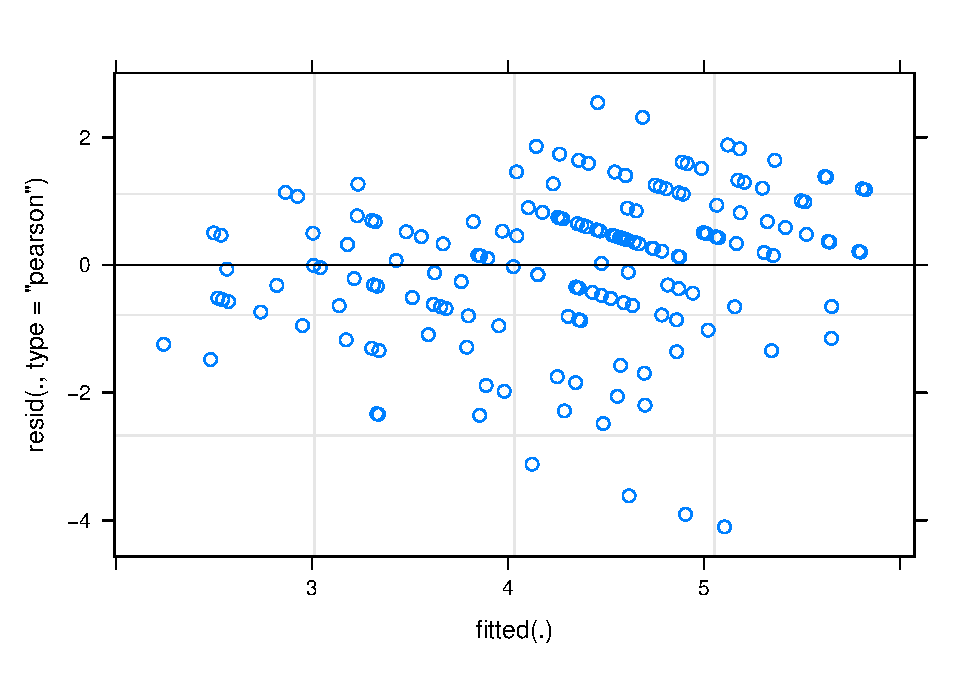
\includegraphics{zoom_sso_manuscript_files/figure-latex/unnamed-chunk-9-1.pdf}

\begin{verbatim}
## Linear mixed model fit by REML. t-tests use Satterthwaite's method [
## lmerModLmerTest]
## Formula: interact_qual ~ daily_SSO + day + (1 | partID)
##    Data: zoom_clean
## 
## REML criterion at convergence: 406.7
## 
## Scaled residuals: 
##      Min       1Q   Median       3Q      Max 
## -3.07232 -0.49077  0.03079  0.58778  2.33422 
## 
## Random effects:
##  Groups   Name        Variance Std.Dev.
##  partID   (Intercept) 0.2450   0.4950  
##  Residual             0.4893   0.6995  
## Number of obs: 167, groups:  partID, 37
## 
## Fixed effects:
##              Estimate Std. Error        df t value Pr(>|t|)    
## (Intercept)   5.14374    0.19094 131.39902  26.939  < 2e-16 ***
## daily_SSO    -0.21801    0.04332 145.86507  -5.033  1.4e-06 ***
## day           0.05243    0.03979 131.63149   1.317     0.19    
## ---
## Signif. codes:  0 '***' 0.001 '**' 0.01 '*' 0.05 '.' 0.1 ' ' 1
## 
## Correlation of Fixed Effects:
##           (Intr) dl_SSO
## daily_SSO -0.615       
## day       -0.668  0.122
\end{verbatim}

Interaction quality (and SSO) and Well-Being

\begin{verbatim}
## Linear mixed model fit by REML. t-tests use Satterthwaite's method [
## lmerModLmerTest]
## Formula: stroop_fatigue ~ interact_qual + daily_SSO + day + (1 | partID)
##    Data: zoom_clean
## 
## REML criterion at convergence: 1099.1
## 
## Scaled residuals: 
##     Min      1Q  Median      3Q     Max 
## -2.5739 -0.5918 -0.1440  0.4195  5.0122 
## 
## Random effects:
##  Groups   Name        Variance Std.Dev.
##  partID   (Intercept)  4.71    2.170   
##  Residual             47.42    6.887   
## Number of obs: 163, groups:  partID, 37
## 
## Fixed effects:
##                Estimate Std. Error        df t value Pr(>|t|)   
## (Intercept)    10.97867    3.91942 144.13734   2.801  0.00579 **
## interact_qual  -0.54378    0.69129 143.93521  -0.787  0.43280   
## daily_SSO       0.04771    0.38992 107.43441   0.122  0.90285   
## day            -0.44295    0.39804 133.39557  -1.113  0.26778   
## ---
## Signif. codes:  0 '***' 0.001 '**' 0.01 '*' 0.05 '.' 0.1 ' ' 1
## 
## Correlation of Fixed Effects:
##             (Intr) intrc_ dl_SSO
## interact_ql -0.910              
## daily_SSO   -0.587  0.404       
## day         -0.222 -0.097  0.031
\end{verbatim}

\begin{verbatim}
## Linear mixed model fit by REML. t-tests use Satterthwaite's method [
## lmerModLmerTest]
## Formula: How_Today ~ interact_qual + daily_SSO + day + (1 | partID)
##    Data: zoom_clean
## 
## REML criterion at convergence: 523.9
## 
## Scaled residuals: 
##     Min      1Q  Median      3Q     Max 
## -2.4678 -0.6050  0.0134  0.6761  2.5977 
## 
## Random effects:
##  Groups   Name        Variance Std.Dev.
##  partID   (Intercept) 0.03099  0.176   
##  Residual             1.24587  1.116   
## Number of obs: 167, groups:  partID, 37
## 
## Fixed effects:
##                Estimate Std. Error        df t value Pr(>|t|)    
## (Intercept)     1.82865    0.60105 136.40386   3.042  0.00282 ** 
## interact_qual   0.50434    0.10548 131.94925   4.781 4.58e-06 ***
## daily_SSO      -0.12378    0.05874  94.15094  -2.107  0.03774 *  
## day             0.12084    0.06298 136.86015   1.919  0.05708 .  
## ---
## Signif. codes:  0 '***' 0.001 '**' 0.01 '*' 0.05 '.' 0.1 ' ' 1
## 
## Correlation of Fixed Effects:
##             (Intr) intrc_ dl_SSO
## interact_ql -0.912              
## daily_SSO   -0.602  0.428       
## day         -0.231 -0.093  0.025
\end{verbatim}

\begin{verbatim}
## Linear mixed model fit by REML. t-tests use Satterthwaite's method [
## lmerModLmerTest]
## Formula: Mental_Fatigue_Daily ~ interact_qual + daily_SSO + day + (1 |  
##     partID)
##    Data: zoom_clean
## 
## REML criterion at convergence: 474.1
## 
## Scaled residuals: 
##     Min      1Q  Median      3Q     Max 
## -2.3978 -0.5890 -0.0573  0.6396  3.4795 
## 
## Random effects:
##  Groups   Name        Variance Std.Dev.
##  partID   (Intercept) 0.5666   0.7527  
##  Residual             0.6714   0.8194  
## Number of obs: 167, groups:  partID, 37
## 
## Fixed effects:
##                Estimate Std. Error        df t value Pr(>|t|)    
## (Intercept)     3.28238    0.54317 162.72993   6.043 9.97e-09 ***
## interact_qual  -0.13737    0.09484 159.85765  -1.448  0.14948    
## daily_SSO       0.28757    0.05749 162.55542   5.002 1.46e-06 ***
## day            -0.12738    0.04703 130.08653  -2.708  0.00767 ** 
## ---
## Signif. codes:  0 '***' 0.001 '**' 0.01 '*' 0.05 '.' 0.1 ' ' 1
## 
## Correlation of Fixed Effects:
##             (Intr) intrc_ dl_SSO
## interact_ql -0.895              
## daily_SSO   -0.564  0.348       
## day         -0.184 -0.106  0.089
\end{verbatim}

\begin{verbatim}
## Linear mixed model fit by REML. t-tests use Satterthwaite's method [
## lmerModLmerTest]
## Formula: SES_daily ~ interact_qual + daily_SSO + day + (1 | partID)
##    Data: zoom_clean
## 
## REML criterion at convergence: 207
## 
## Scaled residuals: 
##      Min       1Q   Median       3Q      Max 
## -2.35540 -0.43496  0.03415  0.56821  2.98927 
## 
## Random effects:
##  Groups   Name        Variance Std.Dev.
##  partID   (Intercept) 0.06438  0.2537  
##  Residual             0.14411  0.3796  
## Number of obs: 167, groups:  partID, 37
## 
## Fixed effects:
##                Estimate Std. Error        df t value Pr(>|t|)    
## (Intercept)     2.52215    0.23914 162.25849  10.547  < 2e-16 ***
## interact_qual   0.08054    0.04202 162.85183   1.917   0.0570 .  
## daily_SSO      -0.10130    0.02495 151.47362  -4.060 7.83e-05 ***
## day             0.05434    0.02169 133.63433   2.505   0.0134 *  
## ---
## Signif. codes:  0 '***' 0.001 '**' 0.01 '*' 0.05 '.' 0.1 ' ' 1
## 
## Correlation of Fixed Effects:
##             (Intr) intrc_ dl_SSO
## interact_ql -0.904              
## daily_SSO   -0.578  0.370       
## day         -0.195 -0.102  0.072
\end{verbatim}

\hypertarget{discussion}{%
\section{Discussion}\label{discussion}}

\newpage

\hypertarget{references}{%
\section{References}\label{references}}

\hypertarget{refs}{}
\begin{CSLReferences}{1}{0}
\leavevmode\vadjust pre{\hypertarget{ref-R-papaja}{}}%
Aust, F., \& Barth, M. (2022). \emph{{papaja}: {Prepare} reproducible {APA} journal articles with {R Markdown}}. \url{https://github.com/crsh/papaja}

\leavevmode\vadjust pre{\hypertarget{ref-bailenson2021nonverbal}{}}%
Bailenson, J. N. (2021). \emph{Nonverbal overload: A theoretical argument for the causes of zoom fatigue}.

\leavevmode\vadjust pre{\hypertarget{ref-R-tinylabels}{}}%
Barth, M. (2022). \emph{{tinylabels}: Lightweight variable labels}. \url{https://cran.r-project.org/package=tinylabels}

\leavevmode\vadjust pre{\hypertarget{ref-R-lme4}{}}%
Bates, D., Mächler, M., Bolker, B., \& Walker, S. (2015). Fitting linear mixed-effects models using {lme4}. \emph{Journal of Statistical Software}, \emph{67}(1), 1--48. \url{https://doi.org/10.18637/jss.v067.i01}

\leavevmode\vadjust pre{\hypertarget{ref-R-Matrix}{}}%
Bates, D., \& Maechler, M. (2021). \emph{Matrix: Sparse and dense matrix classes and methods}. \url{https://CRAN.R-project.org/package=Matrix}

\leavevmode\vadjust pre{\hypertarget{ref-R-purrr}{}}%
Henry, L., \& Wickham, H. (2020). \emph{Purrr: Functional programming tools}. \url{https://CRAN.R-project.org/package=purrr}

\leavevmode\vadjust pre{\hypertarget{ref-R-lmerTest}{}}%
Kuznetsova, A., Brockhoff, P. B., \& Christensen, R. H. B. (2017). {lmerTest} package: Tests in linear mixed effects models. \emph{Journal of Statistical Software}, \emph{82}(13), 1--26. \url{https://doi.org/10.18637/jss.v082.i13}

\leavevmode\vadjust pre{\hypertarget{ref-R-tibble}{}}%
Müller, K., \& Wickham, H. (2021). \emph{Tibble: Simple data frames}. \url{https://CRAN.R-project.org/package=tibble}

\leavevmode\vadjust pre{\hypertarget{ref-pfund2020video}{}}%
Pfund, G. N., Hill, P. L., \& Harriger, J. (2020). Video chatting and appearance satisfaction during COVID-19: Appearance comparisons and self-objectification as moderators. \emph{International Journal of Eating Disorders}, \emph{53}(12), 2038--2043.

\leavevmode\vadjust pre{\hypertarget{ref-R-nlme}{}}%
Pinheiro, J., Bates, D., DebRoy, S., Sarkar, D., \& R Core Team. (2021). \emph{{nlme}: Linear and nonlinear mixed effects models}. \url{https://CRAN.R-project.org/package=nlme}

\leavevmode\vadjust pre{\hypertarget{ref-R-base}{}}%
R Core Team. (2022). \emph{R: A language and environment for statistical computing}. R Foundation for Statistical Computing. \url{https://www.R-project.org/}

\leavevmode\vadjust pre{\hypertarget{ref-R-psych}{}}%
Revelle, W. (2021). \emph{Psych: Procedures for psychological, psychometric, and personality research}. Northwestern University. \url{https://CRAN.R-project.org/package=psych}

\leavevmode\vadjust pre{\hypertarget{ref-R-ggplot2}{}}%
Wickham, H. (2016). \emph{ggplot2: Elegant graphics for data analysis}. Springer-Verlag New York. \url{https://ggplot2.tidyverse.org}

\leavevmode\vadjust pre{\hypertarget{ref-R-stringr}{}}%
Wickham, H. (2019). \emph{Stringr: Simple, consistent wrappers for common string operations}. \url{https://CRAN.R-project.org/package=stringr}

\leavevmode\vadjust pre{\hypertarget{ref-R-forcats}{}}%
Wickham, H. (2021a). \emph{Forcats: Tools for working with categorical variables (factors)}. \url{https://CRAN.R-project.org/package=forcats}

\leavevmode\vadjust pre{\hypertarget{ref-R-tidyr}{}}%
Wickham, H. (2021b). \emph{Tidyr: Tidy messy data}. \url{https://CRAN.R-project.org/package=tidyr}

\leavevmode\vadjust pre{\hypertarget{ref-R-tidyverse}{}}%
Wickham, H., Averick, M., Bryan, J., Chang, W., McGowan, L. D., François, R., Grolemund, G., Hayes, A., Henry, L., Hester, J., Kuhn, M., Pedersen, T. L., Miller, E., Bache, S. M., Müller, K., Ooms, J., Robinson, D., Seidel, D. P., Spinu, V., \ldots{} Yutani, H. (2019). Welcome to the {tidyverse}. \emph{Journal of Open Source Software}, \emph{4}(43), 1686. \url{https://doi.org/10.21105/joss.01686}

\leavevmode\vadjust pre{\hypertarget{ref-R-dplyr}{}}%
Wickham, H., François, R., Henry, L., \& Müller, K. (2021). \emph{Dplyr: A grammar of data manipulation}. \url{https://CRAN.R-project.org/package=dplyr}

\leavevmode\vadjust pre{\hypertarget{ref-R-readr}{}}%
Wickham, H., \& Hester, J. (2020). \emph{Readr: Read rectangular text data}. \url{https://CRAN.R-project.org/package=readr}

\end{CSLReferences}


\end{document}
